\documentclass[a4paper]{article}

\usepackage[latin1]{inputenc} 
\usepackage{graphicx}
\usepackage{natbib}
\usepackage{amsmath}
\usepackage{subcaption}

\usepackage{listings}
\usepackage{color}

% \usepackage{draftwatermark}
%\usepackage{fullpage}

%\SetWatermarkText{
\includegraphics{sw_logo.png}}
\newcommand{\bm}[1]{\mbox{\boldmath{$#1$}}}

\definecolor{codegreen}{rgb}{0,0.6,0}
\definecolor{codegray}{rgb}{0.5,0.5,0.5}
\definecolor{codepurple}{rgb}{0.58,0,0.82}
\definecolor{backcolour}{rgb}{0.95,0.95,0.92}

\lstdefinestyle{mystyle}{
    backgroundcolor=\color{backcolour},   
    commentstyle=\color{codegreen},
    keywordstyle=\color{magenta},
    numberstyle=\tiny\color{codegray},
    stringstyle=\color{codepurple},
    basicstyle=\footnotesize,
    breakatwhitespace=false,         
    breaklines=true,                 
    captionpos=b,                    
    keepspaces=true,                 
    numbers=left,                    
    numbersep=5pt,                  
    showspaces=false,                
    showstringspaces=false,
    showtabs=false,                  
    tabsize=2
}
 
\lstset{style=mystyle}




\begin{document}

\begin{center}
%
\includegraphics[width=0.2\textwidth]{sw_logo} \\
\vspace{0.5 cm}
\huge{\textbf{Python CRootBox Tutorial (py\_rootbox)}} \\
\vspace{0.5 cm}
\normalsize
Daniel Leitner \\
www.simwerk.at 
\end{center}

\vspace{0.5 cm}

\noindent 
The following tutorial offers scripts to outline the usage of the CRootBox Python binding for many different applications. 
For further documentation please refer to the Doxygen class documentation of the CRootBox code.


\vspace{0.5 cm}

\tableofcontents

\newpage



\section{Basic usage}
 
The first example shows how to use CRootBox in the most simple situation: open a parameter file (L7), do the simulation (L13), and save the result (L16). 

\lstinputlisting[language=Python, caption=Example 1a]{../python/example1a.py} % basicstyle=\footnotesize, 

\noindent 
Lets revise the above code in more detail: 
\begin{itemize}
 \item[1] Imports the CRootBox Python library (py\_rootbox), and names it rb.
 \item[3] Constructs the root system object.
 \item[7] Opens two text files: the root type parameter file (.rparam) and the root system parameter file (.pparam). Optionally, as a second argument a path can be provided, the default path is (modelparameter/). 
 Alternatively, all parameter can be set or modified directly in Python (see Section \ref{sec:sa}).
 \item[10] Initializes the simulation: Creates the tap root the base roots (i.e. all basal roots, and shoot borne roots that might emerge), creates the tropisms and passes the domain geometry to it, and creates the elongation functions. 
 \item[13] Performs the simulation. The value 30 is the simulation time in days. If no simulation time is passed the simulation time is taken from the .pparam file. Note that simulation results are independent from the time step, 
 i.e. 30 simulate(1) calls should yield the same result as simulate(30). 
 \item[17] Saves the resulting root system geometry in the VTK Polygonal Data format (VTP) as polylines, see Figure \ref{fig:basicA}. 
\end{itemize}

The next example is an extension of the previous one, where the root system grows in one of two containers (a soil core or rectangular rhizotron).
Such geometries are important if we want to mimic experimental settings. In CRootBox the domain geometry is represented in a mesh free way using signed distance functions (SDF).
A SDF returns the distance to the closest boundary, with negative sign if it lies inside of the domain, and a positive if it the point is outside.

\lstinputlisting[language=Python, caption=Example 1b]{../python/example1b.py}

The geometry is first created by constructing some specialization of the class SignedDistanceFunction, and is passed to the root system by the method setGeometry: 
\begin{itemize}
 \item[12] Construct a soil core. 
 \item[15] Construct a rhizotron.
 \item[18] Pick one of the two geometries. Note that it is important to call setGeometry before initialize.
 \item[30] Its possible to save the geometry as Paraview Python script for visualization, see Figure \ref{fig:basicB}. Run this script in Paraview by Tools$\rightarrow$Python Shell, Run Script.
\end{itemize}

\begin{figure}
\begin{subfigure}[c]{0.5\textwidth}
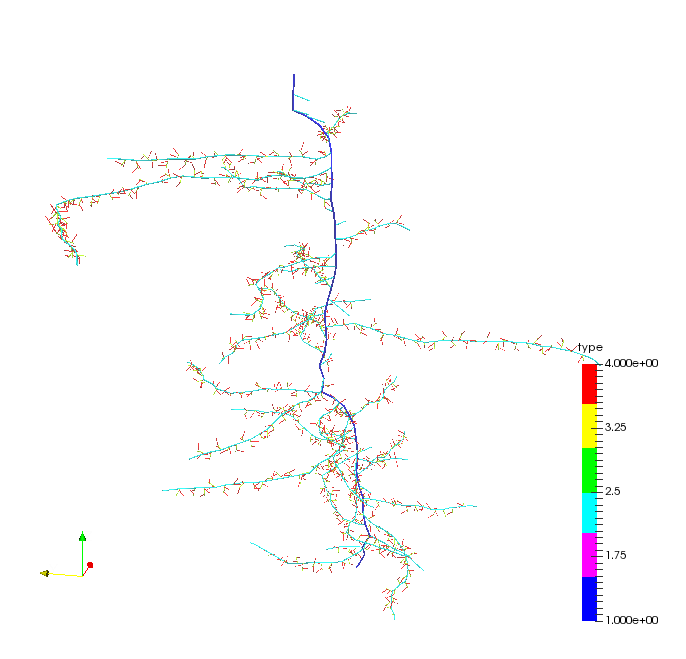
\includegraphics[width=0.99\textwidth]{example_1a.png}
\subcaption{Unconfined growth (Example 1a)} \label{fig:basicA}
\end{subfigure}
\begin{subfigure}[c]{0.5\textwidth}
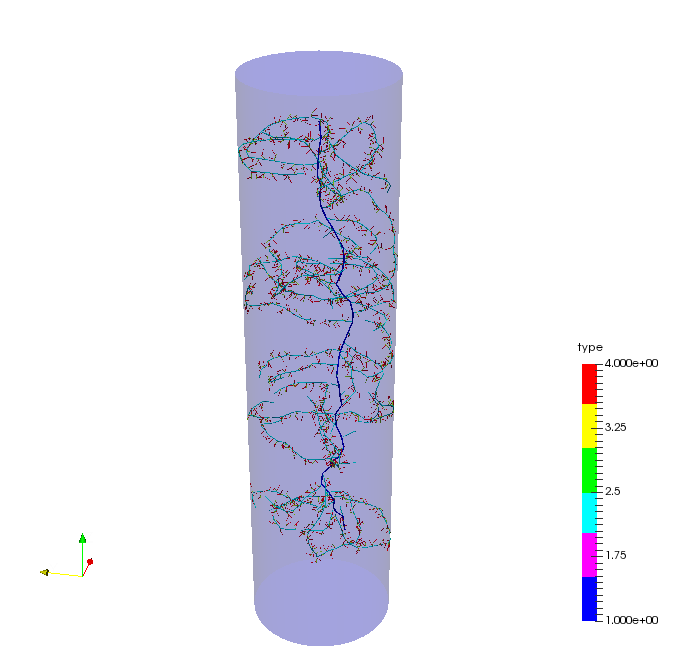
\includegraphics[width=0.99\textwidth]{example_1b.png}
\subcaption{Confined growth (Example 1b)} \label{fig:basicB}
\end{subfigure}
\caption{Resulting figures from Section 1} 
\end{figure}



\section{More complex geometries}

The section shows how to build more complex geometries with SDF. 
Furthermore, we show an example with multiple root systems that is computed in parallel.

\subsection{Using SDF with set operations}

In the following example we create more complex geometries that we might encounter in experiments. 
First, we show how to rotate a rhizotron (e.g. to see more roots at the wall due to gravitropism). 
Second, we create a split box experiment, and finally rhizotubes as obstacles.

The examples show how to build more complex geometries with rotation, translation and using set operations on the SDF.

\lstinputlisting[language=Python, caption=Example 2a]{../python/example2a.py}

\begin{itemize}

\item[10-16] Definition of a rotated rhizotron, see Figure \ref{fig:rhizo}: L12 creates the flat container with a small height, this container is then rotated and translated into the desired position. 
L13 is the position where the origin will lie, and L14 the rotational matrix around the x-axis. 
In L15 the origin position is rotated. Finally, in L16 the new rotated and translated geometry is created. 
 
\item[18-27] Definition of of a split box, see Figure \ref{fig:split}: The split box is composed of a left box, a right box, and a top box connecting left and right. In L27 the geometry is defined by the set operation union of the three compartments. 
 
\item[29-44] Definition of rhizotubes as obstacles, see Figure \ref{fig:rhizotubes}: L30 is the surrounding box, L31 a single rhizotube, that is rotated around the y-axis in L32. L34-L41 create a list of rhizotubes at different locations that mimics the experimental setup. 
L43 and L44 compose the final geometry by to set operation, first a union of all tubes, and then cut them out the surrounding box by taking the difference. 
 
\item[47] Pick one of the three geometries for your simulation.
 
\item[57] Also more complex geometries can be visualized by the Paraview script, however set operations are not really performed, only the involved geometries are visualized.

\end{itemize}

\begin{figure}
\begin{subfigure}[c]{0.3\textwidth}
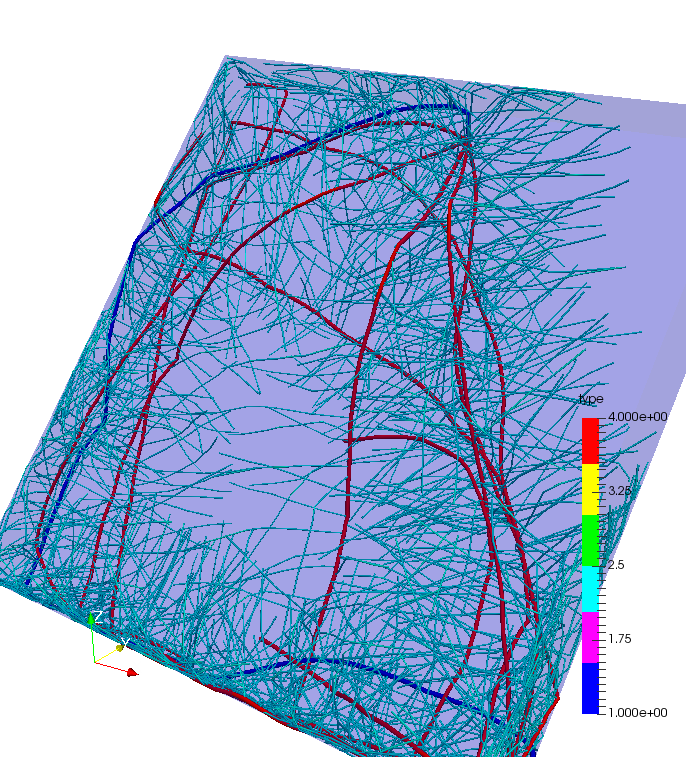
\includegraphics[width=0.99\textwidth]{example_2a1.png}
\subcaption{Rotated rhizotron} \label{fig:rhizo}
\end{subfigure}
\begin{subfigure}[c]{0.3\textwidth}
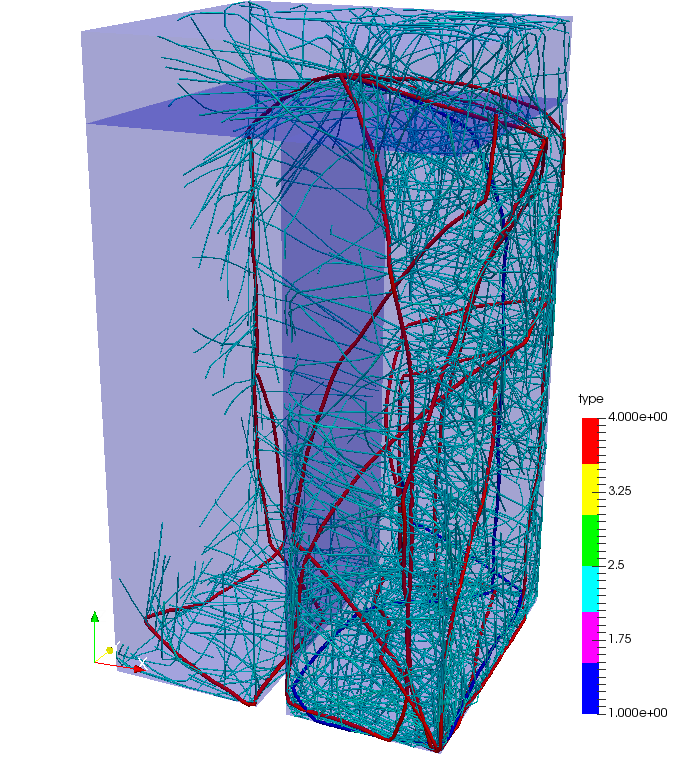
\includegraphics[width=0.99\textwidth]{example_2a2.png}
\subcaption{Split box} \label{fig:split}
\end{subfigure}
\begin{subfigure}[c]{0.3\textwidth}
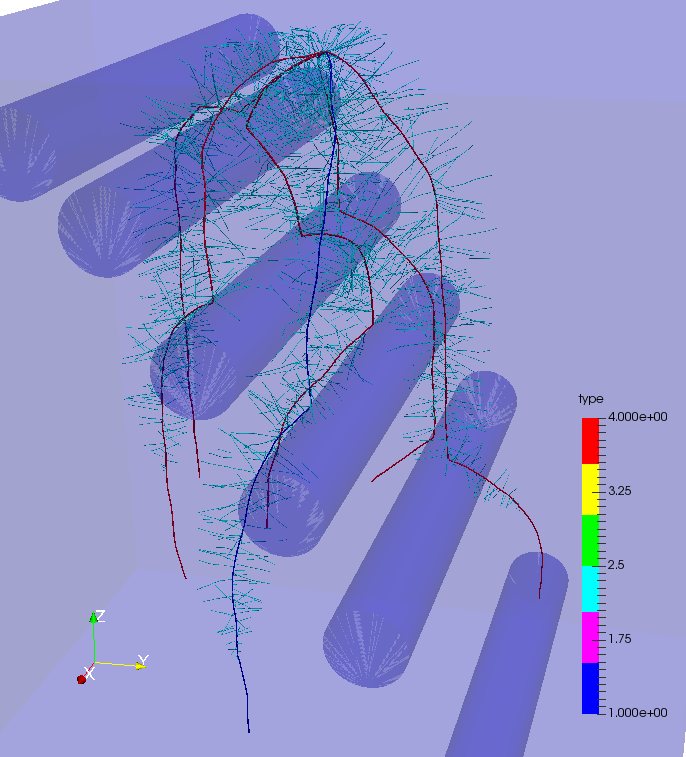
\includegraphics[width=0.99\textwidth]{example_2a3.png}
\subcaption{Rhizotubes} \label{fig:rhizotubes}
\end{subfigure}
\caption{Manipulating SDF (Example 2a)}
\end{figure}



\subsection{Multiple root systems}

Its possible to simulate multiple root systems. In the following we show a small plot scale simulation.

\lstinputlisting[language=Python, caption=Example 2b]{../python/example2b.py}

\begin{itemize}

\item[6,7] Set the number of columns and rows of the plot, and the distance between the root systems.

\item[10-16] Creates the root systems, and puts them into a list allRS. L15 sets the position of the seed. 

\item[20,21] Simulates all root systems 

\item[24-31] Saves each root systems, and additionally, saves all root systems into a single file. 
Therefore, we create an SegmentAnalyser object in L24 and merge all segments into it L28, and finally export the single file L31. The resulting geometry is shown in Figure \ref{fig:multiple}.

\end{itemize}

\begin{figure}
\centering
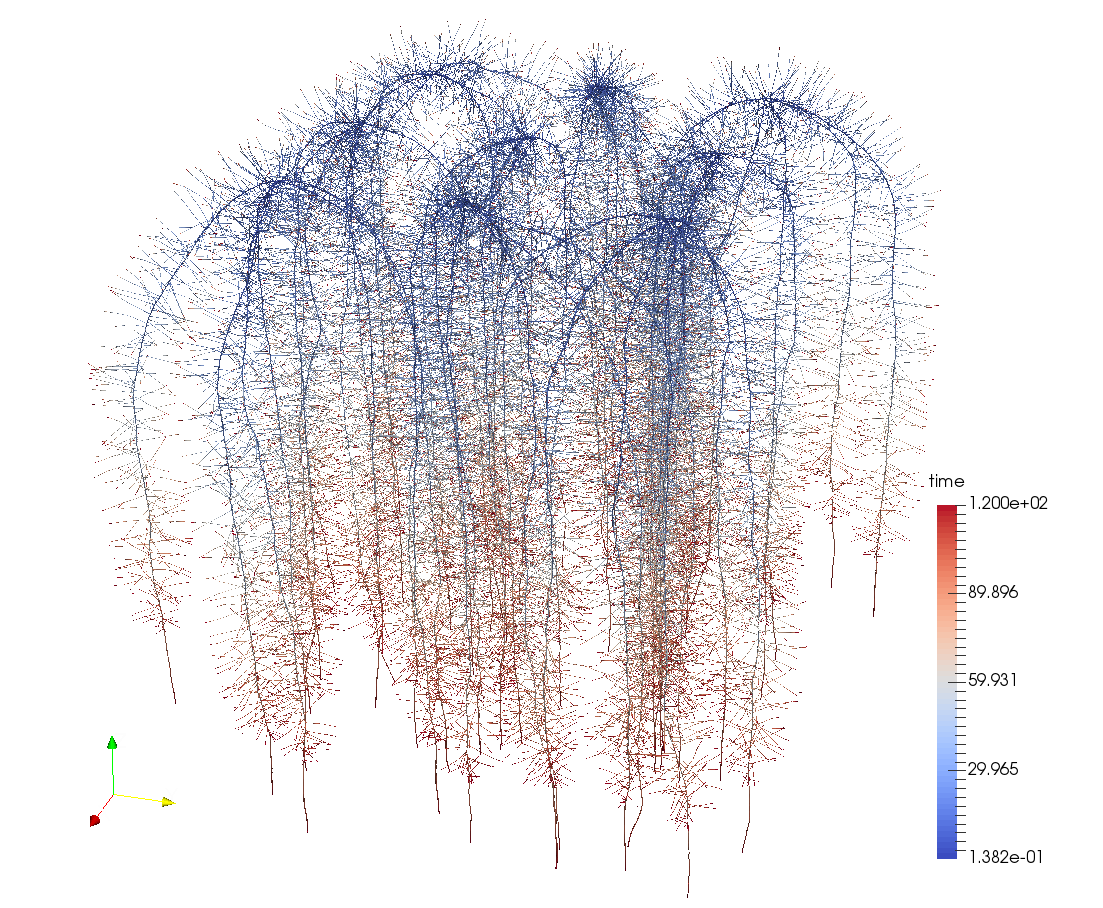
\includegraphics[width=0.7\textwidth]{example_2b.png}
\caption{Multiple root systems (Example 2b), colors denote the creation time of the root segments} \label{fig:multiple}
\end{figure}

Each root system has its own random number generator. By default the seed of the generator is initialized with the system clock. 
If this is not sufficient, e.g. if multiple root systems are initiated at the same time on multi-core systems, or the simulation shall be reproducable, the seed can be set manually using the method RootSystem::setSeed(int).




\section{Analysis of simulation results}

There are various post processing options, on a per root level by the class RootSystem, or a per segment level by the class SegmentAnalyser.
We show some examples of the most frequently used methods. Additionally, we show how model parameters can be modified, 
and how a sensitivity analysis can be performed. 

\subsection{Analysis per root}

The class RootSystem offers some post-processing options. Most of them are on a per root level. 
The following script shows how to analyse length versus time, and how we can obtain root tip or root base positions. 

First, lets analyse the root length versus time, and consider the total root length, and root length per type. 

\lstinputlisting[firstline=1,lastline=41, language=Python, caption=Example 3a (1)]{../python/example3a.py}

\begin{itemize}

\item[2] Rb\_tools is a small utility package that contains functions to convert the exposed C++ data types to NumPy arrays. 
\item[3] NumPy is Python's scientific computing package.
\item[4] Matplotlib is Python's easy way to create figures like in Matlab.

\item[6-9] Sets up the simulation.

\item[11-13] Defines the simulation time, time step, and the resulting number of simulate(dt) calls. 

\item[16,17] First we state which scalar type we want to analyse (others are type, radius, order, time, length, surface, one, parenttype) and in L17 we give it a name for labeling the figure. 

\item[18-21] Pre-definition of the NumPy arrays storing the lengths over time. 

\item[22-29] The simulation loops executes the simulation for a single time step L23. L24 calculates the type of each root, L25 the length (or other scalar type) of the root. 
The functions v2a is defined in the package rb\_tools and converts the C++ vector of doubles to a NumPy array. L26-L29 calculates the total root length in the time step for all roots, and for specific root types.

\item[31-40] Creates Figure \ref{fig:length}.

\end{itemize}

Furthermore, we want to show two options how to retrieve root tip postions and root base positions from a simulation:

\lstinputlisting[firstline=42, language=Python, caption=Example 3a (2)]{../python/example3a.py}

\begin{itemize}

\item[43-44] Reset the simulation and simulate for only 7 days (otherwise there are so many root tips).

\item[46-47] Outputs the number of nodes and segments to get an idea how big the resulting root system is. 
Note that number of segments equals the number of nodes minus the number of base roots that will emerge. Base roots are tap roots, basal roots and shootborne roots.

\item[50-55] The first approach retrieves all roots as polylines L50. Root tips are the last nodes of the polylines L55, root bases the first nodes L54. 
Roots that have not started to grow have only 1 node, and are not retrieved by getPolylines().

\item[58-60] Second approach: L56 returns all nodes of the root system, vv2a converts the vector of the CRootBox C++ type Vector3d to a NumPy array. 
The methods L57, L58 return the indices of the tips and bases. 

\item[63-69] Creates Figure \ref{fig:scatter} using the second approach.

\item[71-73] Verifies that both approaches yield the same result.

\end{itemize}

\begin{figure}
\begin{subfigure}[c]{0.5\textwidth}
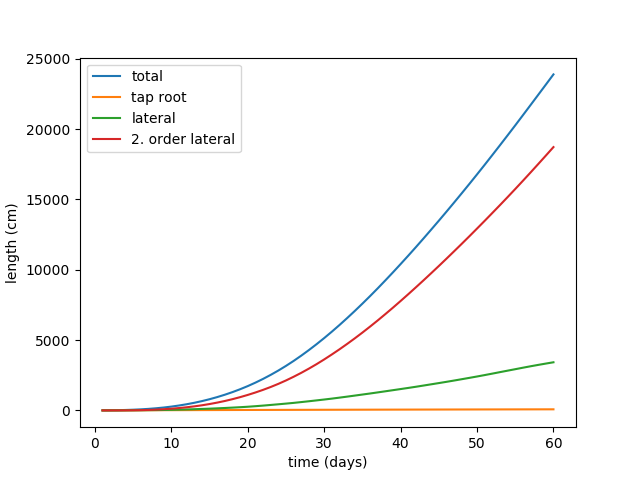
\includegraphics[width=0.99\textwidth]{example_3a.png}
\subcaption{Total root length versus time} \label{fig:length}
\end{subfigure}
\begin{subfigure}[c]{0.5\textwidth}
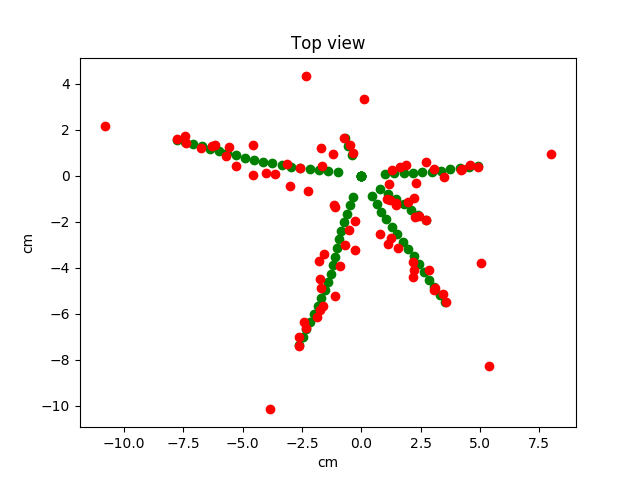
\includegraphics[width=0.99\textwidth]{example_3a2.png}
\subcaption{Top view of the root tip and root bases} \label{fig:scatter}
\end{subfigure}
\caption{Root system analysis (Example 3a)} 
\end{figure}



\subsection{Analysis per segment}

The class SegmentAnalyser offers post-processing methods per root segment. 
The advantage is that we can do distributions or densities, and that we can crop the segments with any geometry for analysis. 
The following script demonstrates some of the possibilities by setting up a virtual soil core experiment. 

\lstinputlisting[language=Python, caption=Example 3b]{../python/example3b.py}

\begin{itemize}

\item[5-L10] Performs the simulation and exports the results.

\item[13-16] We define two soil cores, one in the center of the root and one 10 cm translated. In L16 we pick which one we use for the further analysis.  Figure \ref{fig:soilcoreGeom} shows the resulting geometry.

\item[18-22] Prepares the plot. We use four sub-figures. 

\item[24-28] Creates a root length distribution versus depth. L25 creates the SegmentAnalyser object, and L26 creates the distribution.

\item[30-36] Performs the same distribution in the soil core. In L32 we crop the segments with the geometry. L33 is used to delete unused nodes. 

\item[38-45] Same as before, but we are only interested in segments that are younger than 30 days. In L40 we use the filer method to keep only the segments we want to analyse. 

\item[47-54] The filter method can be used for many different applications. In the following we use it to analyse lateral roots only. Possible rb.ScalarType are: 
'type', 'radius', 'order', segment creation time 'time', 'length', 'surface', 'volume', 'one', 'userdata1', 'userdata2', 'userdata3', and 'parenttype'.
\item[56-58] Show and save resulting Figure \ref{fig:central} or \ref{fig:shifted}.

\end{itemize}

In this example the central core captures only a little amount of laterals (Figure \ref{fig:central}) because the root system is wide spread. 
The shifted root core represents the overall root system slightly better, see Figure \ref{fig:shifted}.  
The basic idea is that such simulations help to increase the understanding of experimental observations.

\begin{figure}
\centering
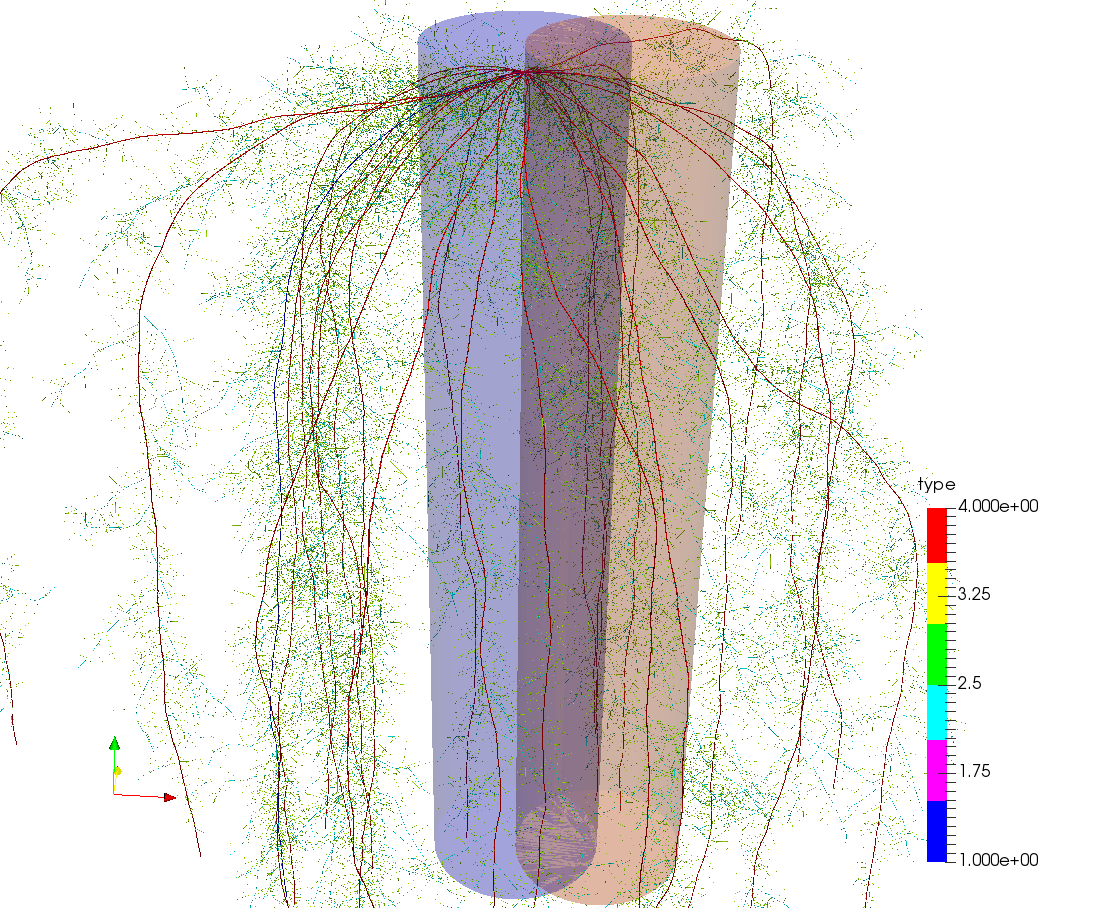
\includegraphics[width=0.6\textwidth]{example_3b.png}
\caption{Virtual soil cores experiment (Example 3b): Central core (blue), shifted core (red)} \label{fig:soilcoreGeom}
\end{figure} 

\begin{figure}
\centering
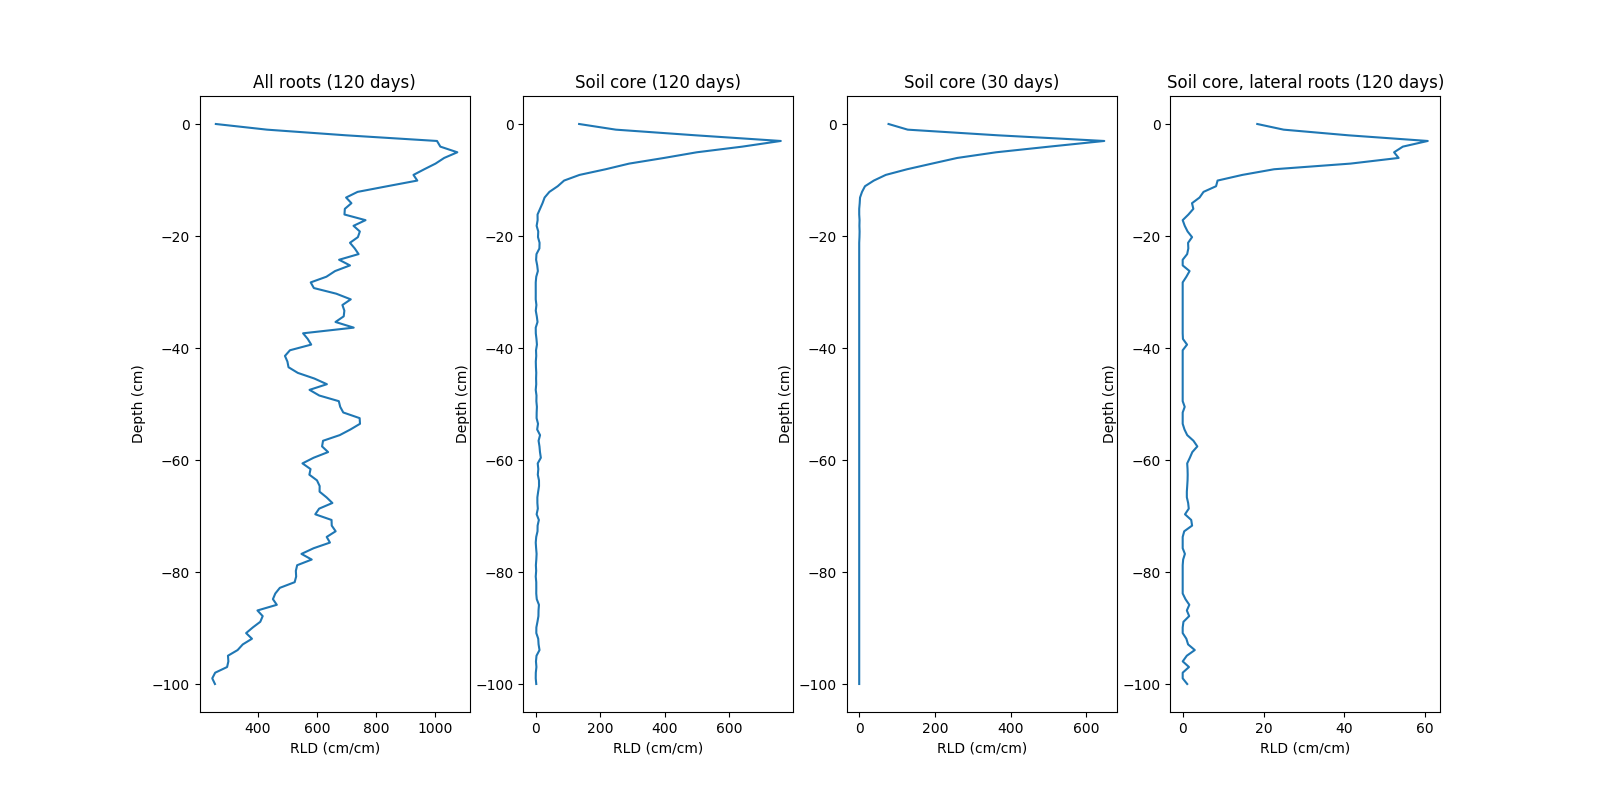
\includegraphics[width=0.9\textwidth]{example_3b1.png} 
\caption{Central core (Example 3b)} \label{fig:central}
\end{figure}

\begin{figure}
\centering
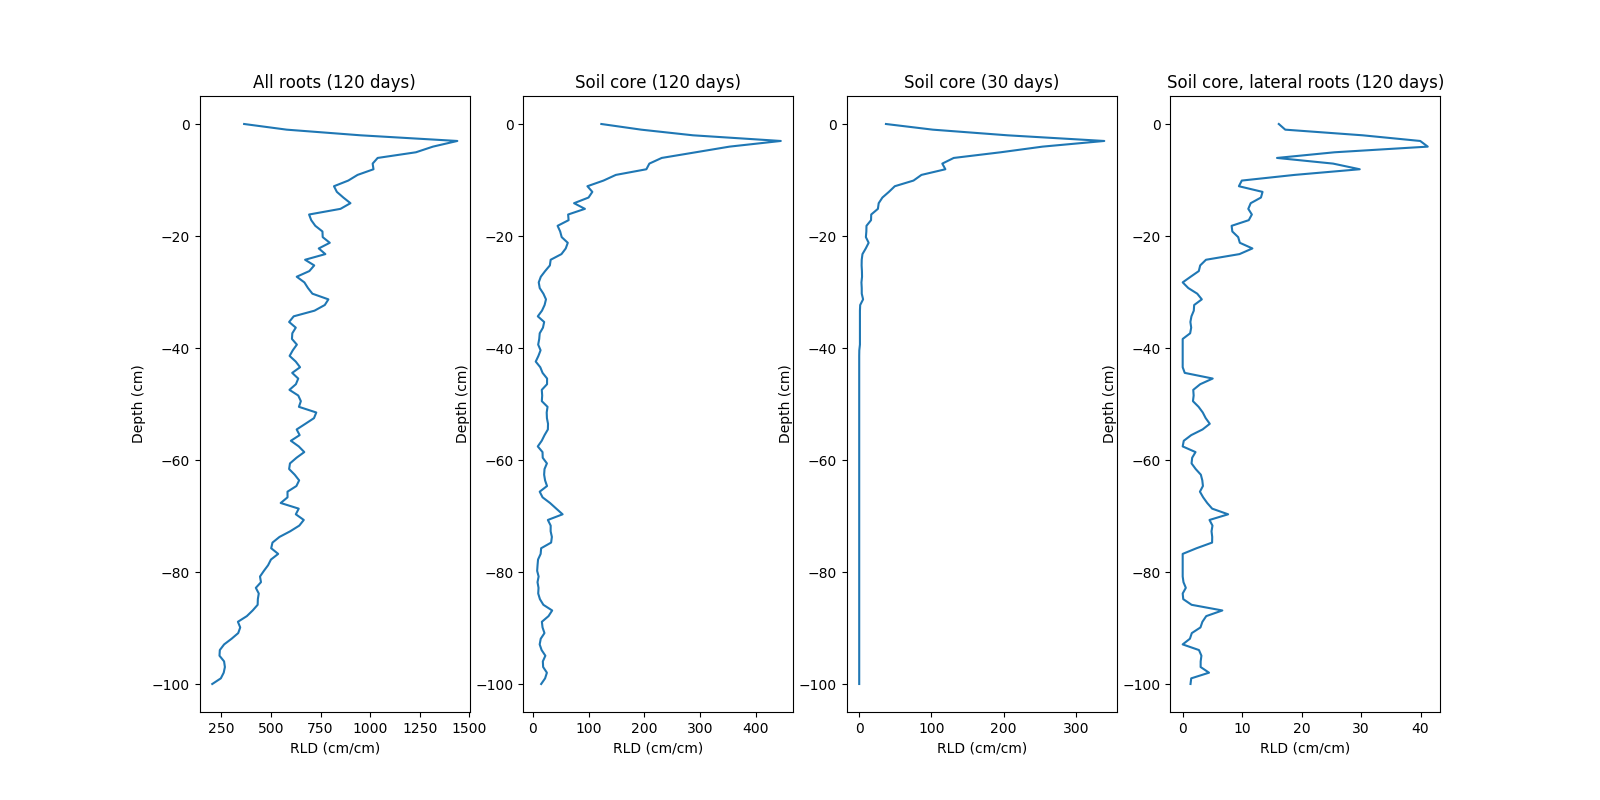
\includegraphics[width=0.9\textwidth]{example_3b2.png} 
\caption{Shifted core (Example 3b)} \label{fig:shifted}
\end{figure}



\subsection{Sensitivity analysis} \label{sec:sa}

In the previous examples we always opened the root system parameters from a file. 
In the following example we show to do everything in a Python script without the need of any parameter files. 
This is especially important if we want to modify the parameters in our scripts like it is needed for sensitivity analysis. 

First we start with a script that defines the parameter within the script, and secondly, we show how we can use this to perform a sensitivity analysis.

\lstinputlisting[language=Python, caption=Example 3c]{../python/example3c.py}

\begin{itemize}

\item[8,9] Create the root type parameters of type 1 and type 2.
\item[11-33] We set up a simple root system by hand. First we define the tap root L11-L24, then the laterals L26-L33. In L20 and L21 we have to convert the Python types to the exposed C++ types.
\item[35,36] Set the root type parameters.

\item[38-43] Create the root system parameter stating when basal and shoot borne roots emerge.

\item[45] Sets the root system parameters.

\item[47-50] Initialize, simulate, export. 

\end{itemize}

Note that all parameters can be set and modified within the script. Especially, standard deviations can be set to zero in order to be able to precisely predict the result. 
For example we can calculate the total root system length analytically, and check if the numerical simulation yield the (exact) same result. 
This is performed in the script benchmark.py, which is used to test and validate CRootBox.

In the next part we vary given parameters in order to make a sensitivity analysis. This takes a lot of simulation runs and we demonstrate the of use parallel computing to speed up execution.
We vary the insertion angle of the tap root and basal root, and look at the change in mean root tip depth and radial distance. 

\lstinputlisting[language=Python, caption=Example 3d]{../python/example3d.py}

\begin{itemize}

\item[8-16] Defines a function to set all standard deviations proportional to the parameter values. We use this function in the following to set the standard deviation to zero everywhere. 

\item[19-23] Parameters of the analysis. $N$ denotes the resolution of the parameter we vary, and $runs$ the number of iterations, i.e. $N\cdot runs$ simulations are performed. 
In L24 we define the insertion angle to be varied linearly between 0 and $\pi/2$.

\item[26-51] Definition of a function that performs the simulation and returns mean root tip depth and radial distance. First we create a root system and set the standard deviation to zero L27-L29. 
L32-L35 sets the insertion angle, tap root is always of type 1, and in the parameter file basal roots are of type 4. L38-39 performs the simulation. 
L42-L49 calculates the mean root tip depth and radial distance. 

\item[53-69] This section performs the computation. L53-54 preallocates the resulting arrays. L58-L64 performs the parallel computations, index $i$ is the index of the insertion angle. L67-L69 calculates the mean values.

\item[72-82] Creates the resulting Figure \ref{fig:sa}

\end{itemize}

\begin{figure}
\centering
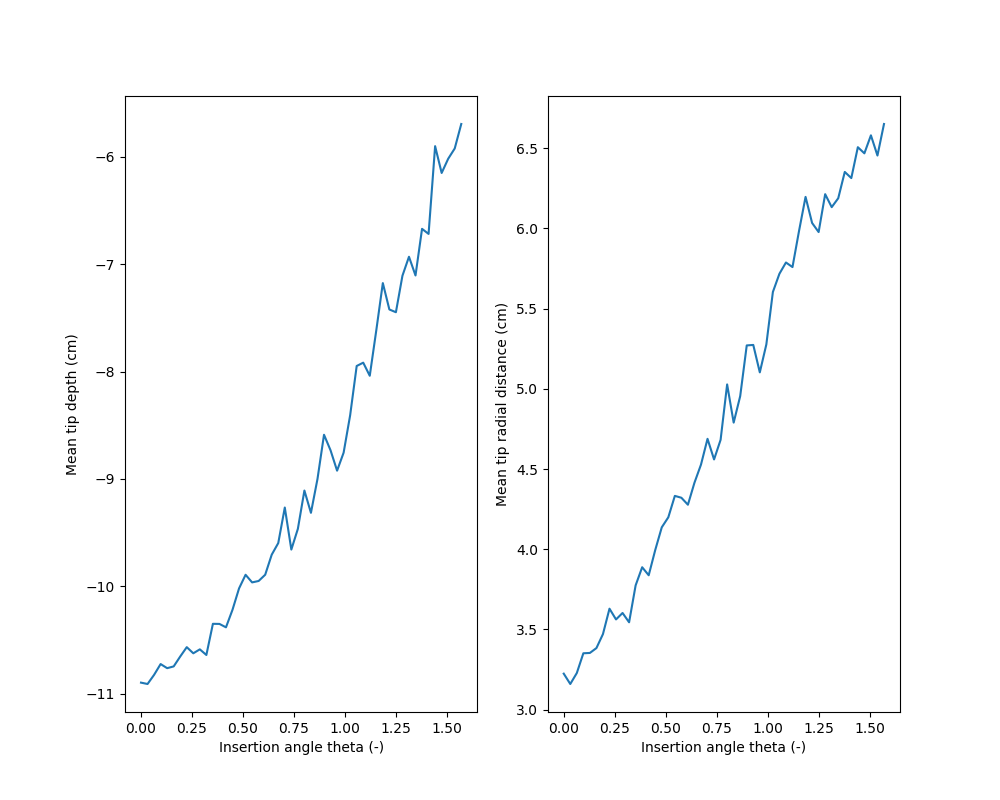
\includegraphics[width=0.7\textwidth]{example_3d.png}
\caption{Sensitivity of mean root tip depth (left) and radial distance (right) to the insertion angle theta (Example 3d) } \label{fig:sa}
\end{figure}



\subsection{How to make an animation}

In order to create an animation in Paraview we have to consider some details. 
The main idea is to export the result file as segments using the class SegmentAnalyser. 
A specific frame is then obtained by thresholding within Paraview using the segments creation times. 

We modify example1b.py to demonstrate how to create an animation.

\lstinputlisting[language=Python, caption=Example 3e (modified from Example 1b)]{../python/example3e.py}

\begin{itemize}

\item[14-16] Its important to use a small resolution in order to obtain a smooth animation. L16 set the axial resolution to 0.1 cm. 

\item[23] Instead of saving the root system as polylines, we use the SegmentAnalyser to save the root system as segments.

\item[26] We save the geometry as Python script for the visualization in ParaView.

\end{itemize}

After running the script we perform the following operations to create an animation:
\begin{enumerate}
 \item Open the .vtp file in ParaView (File$\rightarrow$Open...).
 \item Optionally, create a tube plot with the help of the script scripts/tubePlot.py (Tools$\rightarrow$Python Shell, press 'Run script').
 \item Optionally, visualize the domain boundaries by running the script results/example\_3e.py (Tools$\rightarrow$Python Shell, press 'Run script').
 \item Run the script scripts/animate.py (Tools$\rightarrow$Python Shell, press 'Run script'). The script creates the threshold filter and the animation. 
 \item Use File$\rightarrow$Save Animation... to render and save the animation.
\end{enumerate}



\section{Root functional modelling}

Root growth is strongly influenced by pedo-climate conditions, and plant internal state. CRootBox offers build in ways to develop such models. 
In this section we assume static soil conditions, and describe predefined ways how the soil can affect root growth.
Dynamic soil conditions are described in the following section 'Coupling with a soil model'. 

Implemented root responses are (1) the change in direction of the growing root tip, described in Sections \ref{sec:hydro} and \ref{sec:usertropism} 
(2) the scaling of the elongation rate (3) the change of insertion angle (4) the change of lateral emergence probability, (2)-(4) are described in Section \ref{sec:elongation}.

\subsection{Hydro- and chemotropism} \label{sec:hydro}

Root growth direction is influenced by soil conditions such as water content, soil strength, or nutrient concentration. 
In the following we show how this is achieved in CRootBox.

\lstinputlisting[language=Python, caption=Example 4a]{../python/example4a.py}

\begin{itemize}

\item[3-5] Creates the root system and opens the parameter file

\item[7-14] Change the tropism for the first ten root types: L10 retrieves the parameter, where the CRootBox parameters run from 1 to 11. L11 modifies the axial resolution, and L12-14 sets the three tropism parameters. 

\item[16-22] Definition of a static soil property using SDF. We first define the geometry (L20-L21), and then create a static soil (L22) that obtains the maximal value $maxS$ inside the geometry, 
$minS$ outside the geometry, and linear slope with length $slope$. At the boundary the soil has the value $(maxS+minS)/2$.

\item[25] Sets the soil. Must be called before RootSystem::initialize()

\item[28] Initializes the root system, and among others sets up the hydrotropism. 

\item[30-36] Simulation loop

\item[39] Exports the root system geometry

\item[42-43] We actually do not wish to set this geometry, but we abuse the writer of the class RootSytem to export a Python script showing the layer geometry. The resulting ParaView visualization is presented in Figure \ref{fig:chemo}.

\end{itemize}

\begin{figure}
\centering
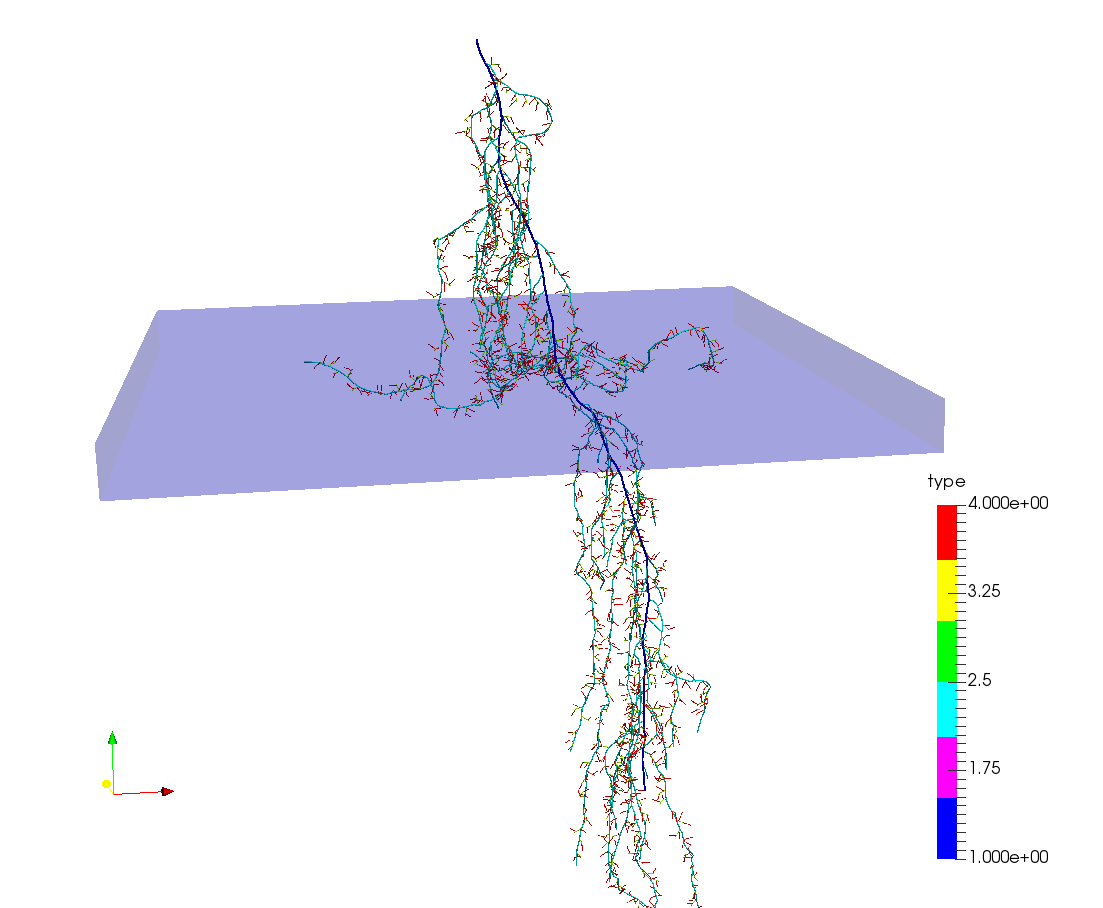
\includegraphics[width=0.7\textwidth]{example4a.png}
\caption{Chemotropism in a nutrient rich layer (Example 4a)} \label{fig:chemo}
\end{figure}



\subsection{User defined tropisms} \label{sec:usertropism}

Normally, the simulation is created from a set of parameters. For tropisms these are the type of tropism $tt$, number of trials $N$ , and tortuosity $\sigma$.
There are two ways to add user defined tropisms: 

\begin{enumerate}
\item The first is C++ only: It is to extend the CRootBox class and overwrite the method RootSystem::createTropism. 
This is the function that is called, when the tropisms are created from the parameters ($tt$, $N$, $\sigma$) in RootSystem::initialize(). 
This is necessary when user defined tropism are created from a parameter file, where $tt$ is the number of the new tropism type. 
\item The second is to manually set the tropisms using the method RootSystem: :setTropism. Make sure to call Rootsystem::setTropism($\dots$) after Rootsystem::initialize().
\end{enumerate}

In both approaches the user has to extend the new tropism class from the class Tropism. 
If just the objective function of the tropism is changed, it is enough to overwrite Tropism::tropismObjective. 
This can done in Python or in C++,the classes Hydrotropism, Gravitropism, and Plagiotropism are examples for this procedure.

If the whole concept of the random optimization is altered, Tropism: :getUCHeading must be overwritten. 
If the geometry model is also changed Tropism: :getHeading must be overwritten.

The following example shows how to implement a new tropism in Python. Two new tropism are introduced:
The first does nothing put to output the incoming arguments of the method Tropism::tropismObjective to the command line (e.g. for debugging).  
The second one, is a Plagiotropism that changes with time to Gravitropism depending on the root age.

\lstinputlisting[language=Python, caption=Example 4b]{../python/example4b.py}

\begin{itemize}

\item[3-14] Creates a new tropism that just writes incoming arguments of Tropism: :tropismObjective to the command line. This can be used for debugging. The new class is extended from rb.Tropism, 
and the method Tropism::tropismObjective is overwritten with the right number of arguments.

\item[16-32] Again, we extend the new class from rb.Tropism. In L19-24 we define our own constructor.
Doing this two things are important: (1) the constructor of the super class must be called (L20), and (2) the tropism parameters $n$, and $\sigma$ must be set (L23). 
Furthermore, the constructor defines two tropisms: plagio- and gravitropism, that are used in Tropism::tropismObjective at a later point, and a root age, when to switch from plagi- to gravitropism. \\
In L26-L32 the method Tropism::tropismObjective is defined. We choose the predefined objective function depending on the root age.

\item[34-38] Sets up the simulation.

\item[40-44] L40,L41 creates the first user defined tropsim. Since we did not define a constructor Tropism::setTropismParameter must be called. L43 creates the second user defined tropism. 
In L44 the tropism is chosen, using the method Tropism::setTropism. The second argument states for which root type it applies. 
Number 2 is the root type number of the laterals, -1 states that the tropism applies for all root types (default = -1).

\item[46-51] The simulation loop. 

\item [54] Exports the result producing Figure (\ref{fig:tropism}). Comparing to Figure (\ref{fig:basicA}) we can see the effect of the new user defined tropsim.

\end{itemize}

\begin{figure}
\centering
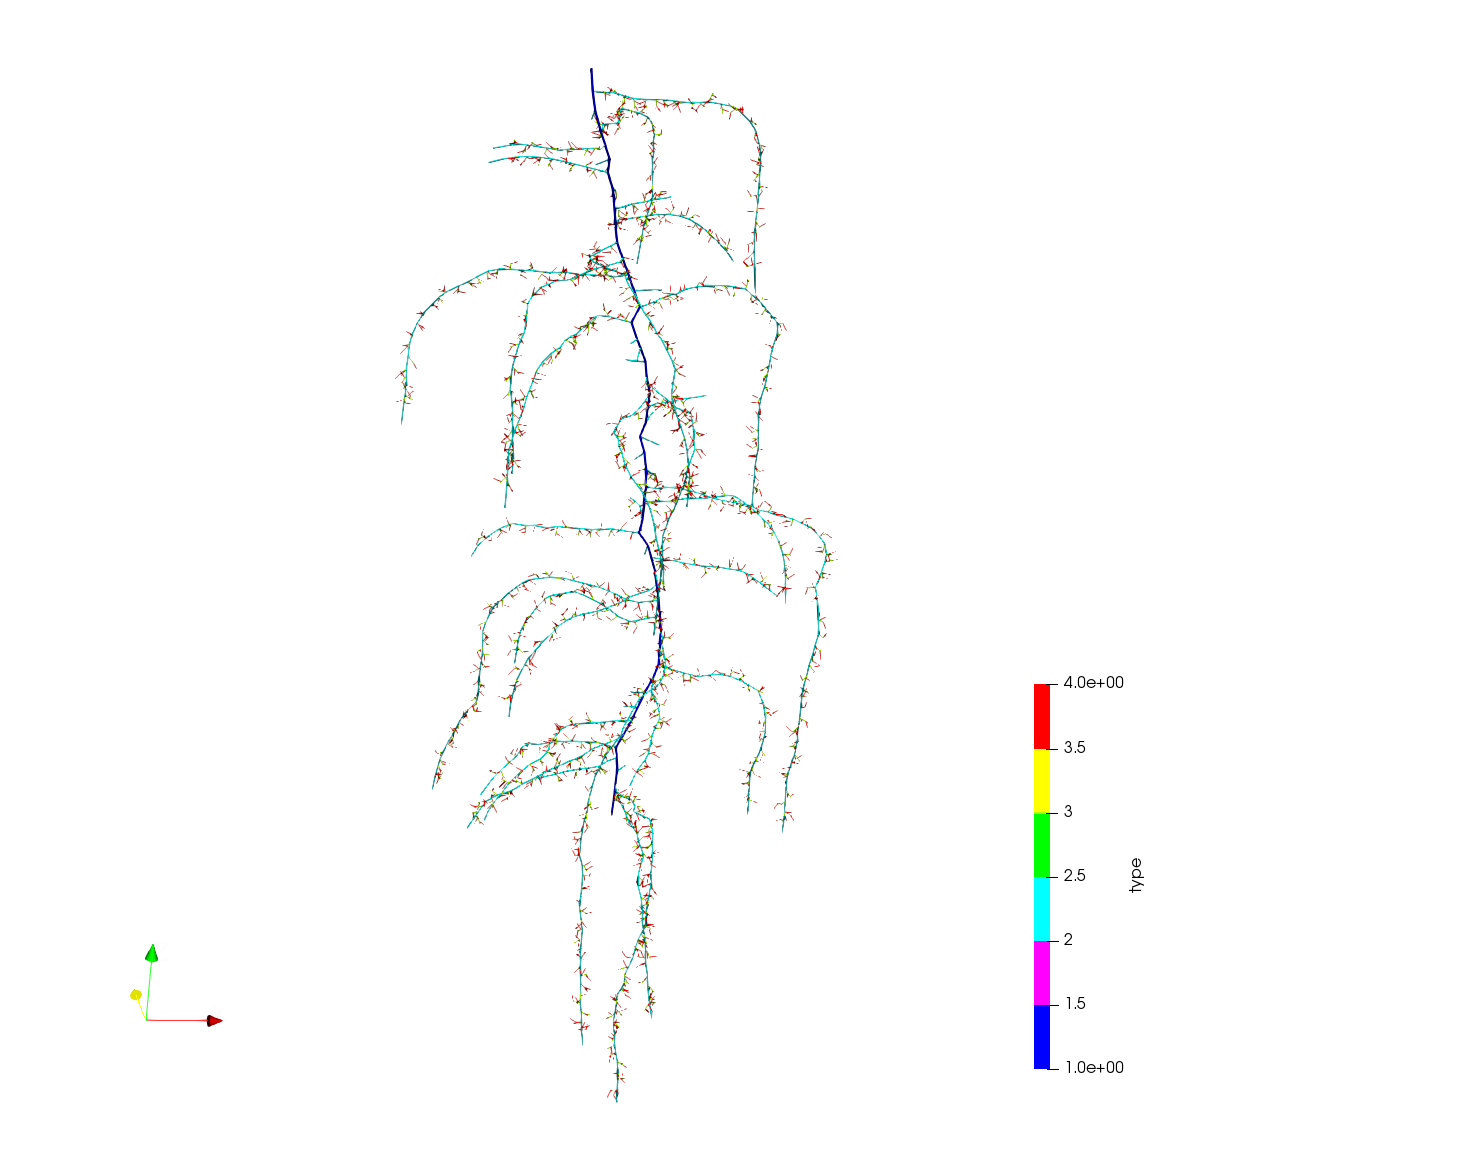
\includegraphics[width=0.7\textwidth]{example4b.png}
\caption{Depending on root age the laterals follow plagio- or gravitropism (Example 4b)} \label{fig:tropism}
\end{figure}



\subsection{Scaling elongation rate, insertion angle, and lateral emergence probability} \label{sec:elongation}

The following script is an example to this and the following two sections, where (a) the elongation rate, (b) the insertion angle, and (c) the probability of lateral emergence are scaled.

Without giving a specific model these mechanisms are considered important. 
For example the elongation rate as well as the probability of lateral emergence is dependent on soil properties like water saturation, soil strength, and temperature (among others).  
The insertion angle is reported to be dependent on nutrient supply in some species. Furthermore, theses mechanisms are influenced by plant systemic responses.

The scaling itself can be performed in the following way:

\lstinputlisting[firstline=1,lastline=50, language=Python, caption=Example 4c (1)]{../python/example4c.py}

\begin{itemize}

\item[4-6] Creates the root system and opens the parameter file

\item[8-13] We create a confining box with two overlapping boxes left and right. This geometries are used for later analysis.

\item[15-21] We define two static soil properties using SDF (L20, L21) as explained in Section \ref{sec:hydro}. 
The left compartment has the value $minS$, the right $maxS$, between them is a linear gradient of length $slope$.

\item[23-34] Sets the scaling functions. L24-L28 adjusts axial resolution and tortuosity $sigma$. L31 sets the scale elongation function $se$ to the soil property. L34 sets the scale insertion angle function $sa$. 
Comment and uncomment the relevant code parts to achieve the desired scaling, to achieve the resulting Figures \ref{fig:elongation} and \ref{fig:insertion}.

\item[36-41] Sets the lateral emergence probability. 
First, we increase the number of laterals of the first laterals (root type 2) by a factor of five and decrease the inter-nodal distances for the same factor L37-L39. This is the maximal lateral density that can be achieved.
Then, we set the scale branching probability function $sbp$ to the soil property defined in L21, see Figure \ref{fig:probability}.

\item[44-49] Initialization and simulation loop.

\end{itemize}

\begin{figure}
\begin{subfigure}[c]{0.3\textwidth}
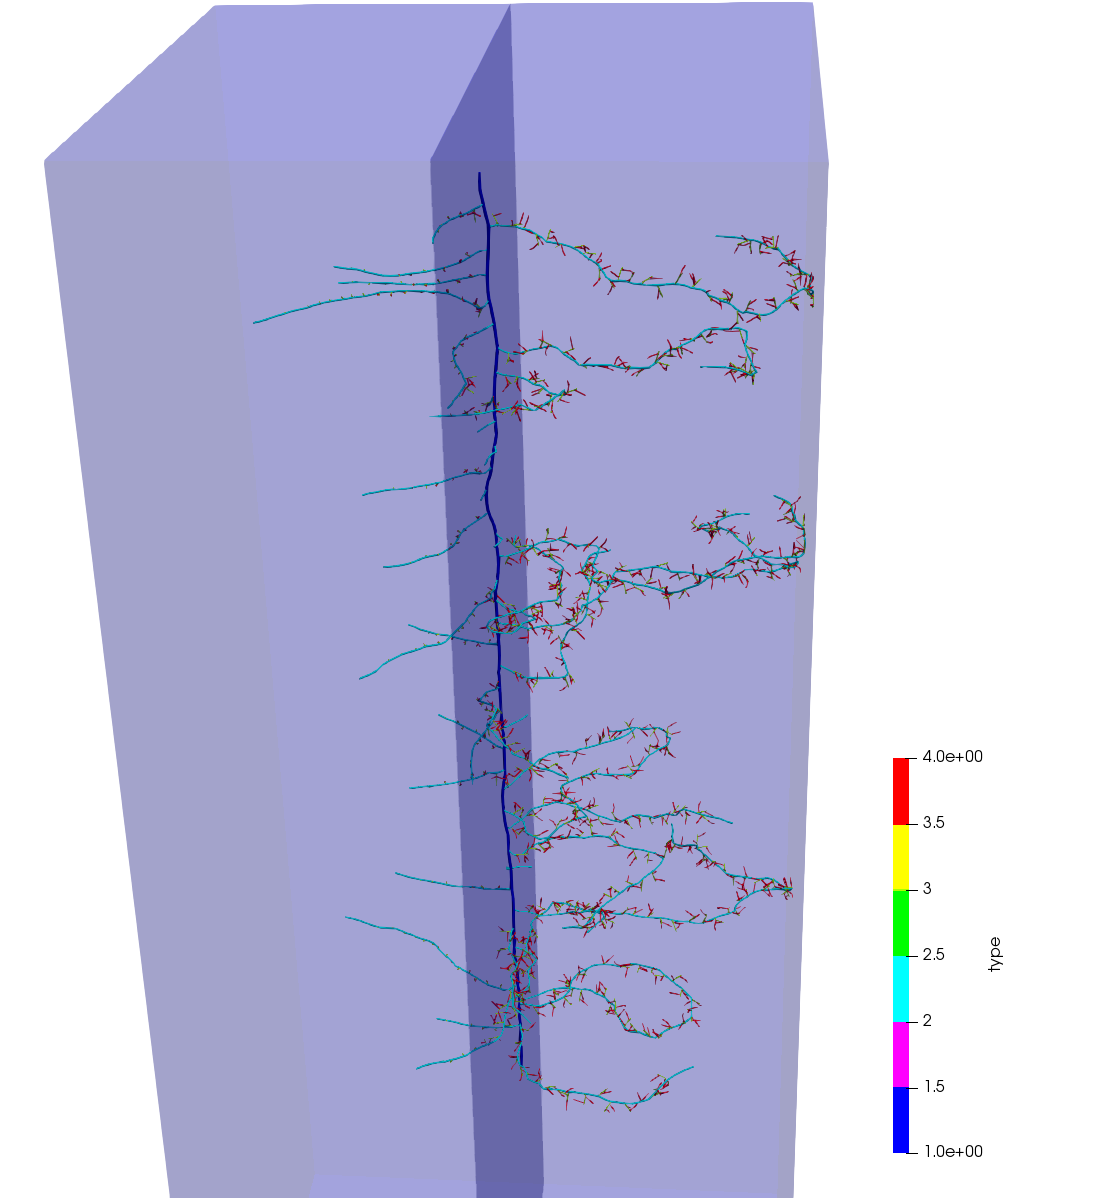
\includegraphics[width=0.99\textwidth]{example4c1.png}
\subcaption{Root elongation rate} \label{fig:elongation}
\end{subfigure}
\begin{subfigure}[c]{0.3\textwidth}
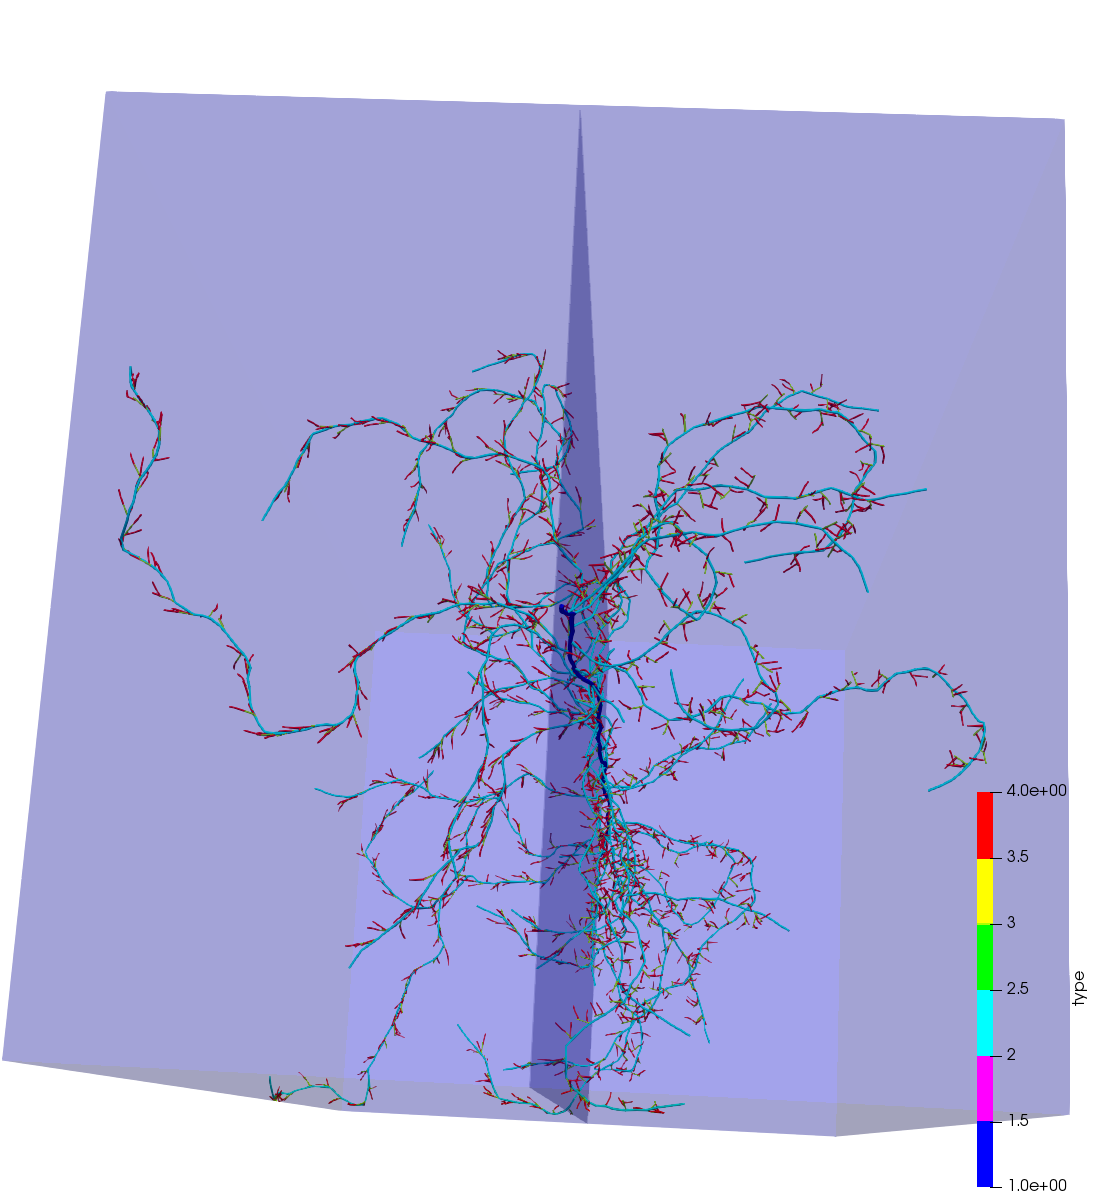
\includegraphics[width=0.99\textwidth]{example4c2.png}
\subcaption{Insertion angle of laterals} \label{fig:insertion}
\end{subfigure}
\begin{subfigure}[c]{0.3\textwidth}
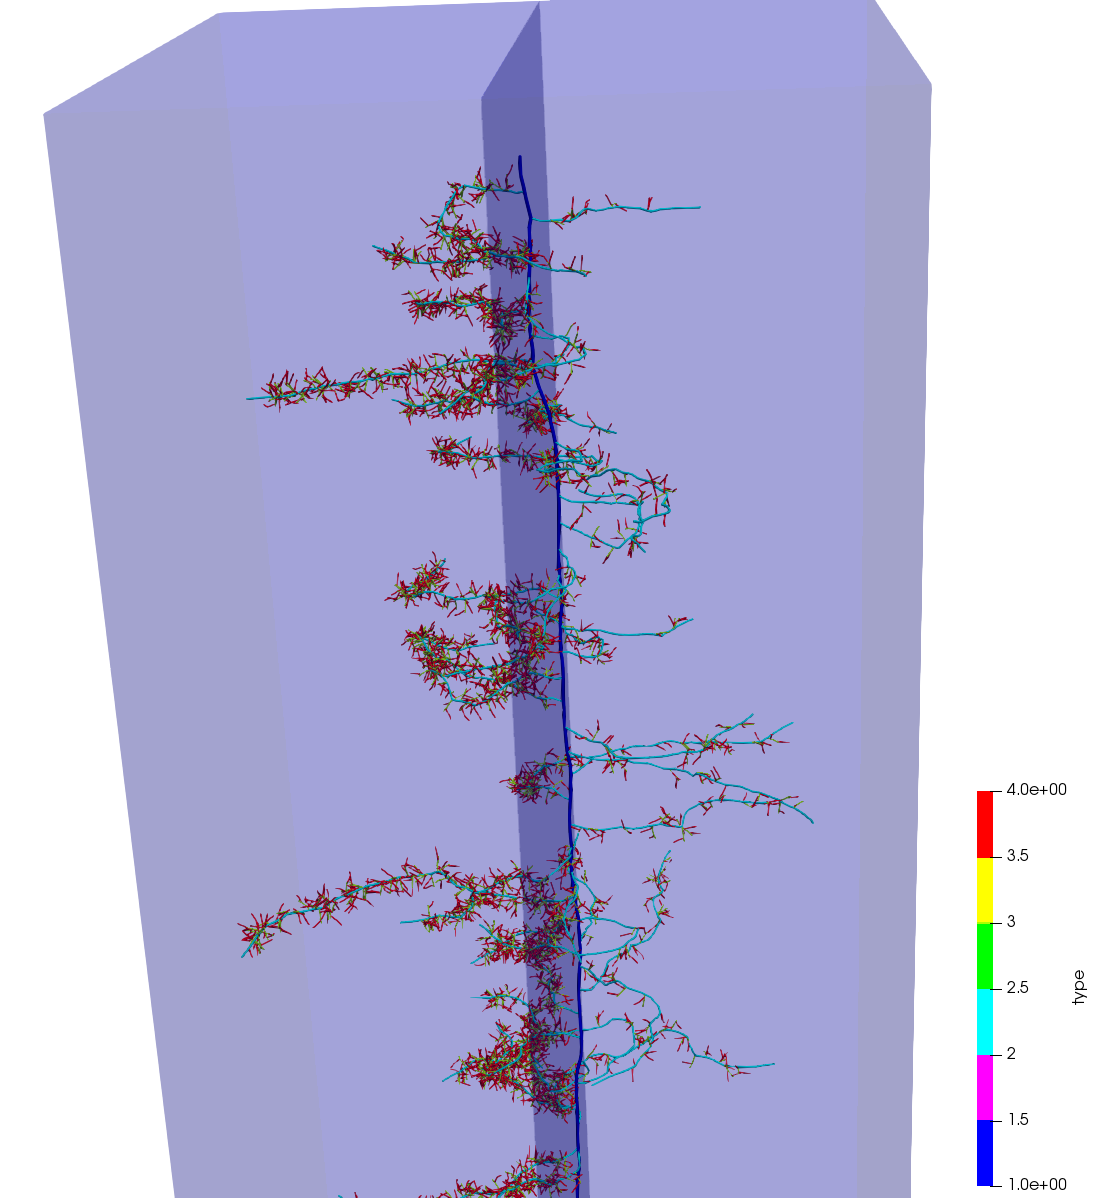
\includegraphics[width=0.99\textwidth]{example4c3.png}
\subcaption{Branching density (probabilistic model)} \label{fig:probability}
\end{subfigure}
\caption{Predefined root responses (Example 4c)}
\end{figure}

When playing with model parameters, it is not always clear if the suggested effect is realized from the figures alone. The following script helps to quantify the effects of above simulation: 

\lstinputlisting[firstline=51,lastline=81, language=Python, caption=Example 4c (2)]{../python/example4c.py}



\section{Model coupling}

In the previous section root responses were described in a static soil. 
In this section we will extend this to a dynamic soil setting, where we update the soil in the simulation loop, and then update the root system iteratively for small time steps. 

General properties of the soil, are passed to the root model via a look up method SoilLookUp::getValue in the class SoilLookUp. 
In the following subsection we will first describe this metod and some implemented usefull extensions of the SoilLookUp class (Section \ref{sec:soil}), 
and show how we can create an interface to a generic soil in Pyhton (Section \ref{sec:usersoil}). 

Next, we show how we can use the soil representation to implement fully coupled models. First we discuss how to obtain a graph representation of the root system, and solve water flow within the root system. 
Then we discuss the example published in \cite{}. 

Finally, we present features that can be used to analyse the dynamic behaviour of the root system development.



\subsection{Soil} \label{sec:soil}


\subsection{User defined soil} \label{sec:usersoil}




\subsection{Graph representation} \label{sec:graph} 

In this section we show how to build an adjacency matrix, and how to calculate fluxes within the root system.

\lstinputlisting[language=Python, caption=Example 5a]{../python/example5a.py}

\subsection{Coupling to 1D water content} \label{sec:fullcoupling} 

Explain and link to paper example (to do)



\subsection{Other dynamic aspects} \label{sec:published}

In this section it is described how information about the last time step can be retrieved, 
and how we can incrementally obtain the root system from only new nodes and segments. 
These methods are especially important if we couple to other numerical software like DuMux (example 5b)



\lstinputlisting[firstline=1, lastline=58, language=Python, caption=Example 5b]{../python/example5b.py}

\bibliographystyle{apalike}
\bibliography{references}


\end{document}
